% ---------------------------------------------------------------------
% HEADER
% Formålet med å legge header til et eget dokument er å garantere at
% oppsettet av dokumentene er likt for alle løsningsforslagene.
% I headeren skjer følgende:
% (1) Dokumentet blir startet
% (2) Pakker blir importert
% ---------------------------------------------------------------------
% ---------------------------------------------------------------------
% HEADER
% Formålet med header er å importere de samme pakkene i alle dokumentene.
% ---------------------------------------------------------------------

% Sett opp dokumentet. Her kan 'twoside' brukes for printing
\documentclass[12pt, a4paper]{article}

% Vi trenger utf-8 for å bruke norske bokstaver: Æ, Ø, Å
\usepackage[utf8]{inputenc}

% Vi setter babel til norsk, da får dokumentegenskaper norske titler
\usepackage[norsk]{babel}

% For å kunne bruke grafikk
\usepackage{graphicx}
\newcommand{\figwidth}{0.75}

% Matematikkpakker fra AMS - American Mathematical Society
\usepackage{amsmath, amsthm, amsfonts, amssymb, mathtools}

% For eventuelle linker, e.g. \href{URL}{text}
\usepackage{hyperref}

% For headers og footers med eventuell logo
\usepackage{fancyhdr}

% Sett marginer manuelt
\usepackage[top = 3cm, left = 3cm, right = 3cm, bottom = 3cm]{geometry}

% For enkle lister, nyttig for oppgave a), b), c), ...
\usepackage[sharp]{easylist}

% Dersom flere kolonner er ønskelig i deler av dokumentet
\usepackage{multicol}

% For luft mellom paragrafer
\usepackage{parskip}

% For logikk assosiert med logoer
\usepackage{ifthen}

% For å finne totalt antall sider
\usepackage{lastpage}

% Annet
\usepackage{enumitem}

\usepackage{polynom}% Polynomer
\polyset{style=C, div=:}

\usepackage{systeme}% Likningssystemer

% Kan brukes når noe stryker ut noe, f.eks 1/n * n, her kan man ta \frac{1}{\cancel{n}} * \cancel{n}
\usepackage{cancel}



% ---------------------------------------------------------------------
% DOKUMENTVARIABLER
% ---------------------------------------------------------------------
\newcommand{\fagkode}{S2}
\newcommand{\semesteraar}{våren 2016}
\newcommand{\forfatter}{Tommy O.}
\newcommand{\dokumenttittel}{Løsningsforslag -- Eksamen \fagkode, \semesteraar}


% Set til 'true' og oppgi logo dersom du vil bruke en logo
\newboolean{bruklogo}
\setboolean{bruklogo}{false}
\newcommand{\logonavn}

% ---------------------------------------------------------------------
% SETUP
% Formålet med å legge setup til et eget dokument å garantere at headers,
% footers, og øverste del av dokumentet er likt for alle
% løsningsforslagene.
% ---------------------------------------------------------------------
% ---------------------------------------------------------------------
% HEADER
% Formålet med setup er at dokumentene ser rimelig like ut.
% ---------------------------------------------------------------------


% ---------------------------------------------------------------------
% Alternativ font. Kommentert ut fordi Computer Modern (default) er pen
%\usepackage{kmath,kerkis}
%\usepackage[T1]{fontenc}
% ---------------------------------------------------------------------


% ---------------------------------------------------------------------
% Sett opp headers og footers
\ifthenelse{\boolean{bruklogo}}{
% Dersom logo skal brukes, sett logoen oppe til høyre med bredde 4 cm
	\rhead{\includegraphics[width=3.5cm]{\logonavn}}
}{
% Dersom logo ikke skal brukes, sett tom header
	\rhead{}
} 
\rfoot{\thepage}
\cfoot{}
\lhead{}
\lfoot{{\scriptsize Forbedringsforslag? Bidra på \url{https://github.com/tommyod/matte_eksamener_VGS}.}}
\renewcommand{\headrulewidth}{0pt}
% ---------------------------------------------------------------------


% ---------------------------------------------------------------------
% To streker under svaret
\def\answer#1{\underline{\underline{#1}}}
% ---------------------------------------------------------------------


% ---------------------------------------------------------------------
% Start selve dokumentet
% ---------------------------------------------------------------------

\begin{document}
\pagestyle{fancy}
{\bfseries \Large \dokumenttittel} \\
{ \footnotesize Laget av \forfatter 
	\hfill Sist oppdatert: \today 
	\hfill Antall sider: \pageref*{LastPage}}
\hrule
\vspace{1em}
\begin{center}
\fbox{\fbox{\parbox{.90\textwidth}{
	Dette dokumentet er open-source;
	alle kan bidra til å gjøre det bedre.
	Dersom du finner skrivefeil, matematiske feil, eller ser at forklaringene kan være bedre: ikke nøl med å sende inn en endring. 
	Du kan finne siste versjon, og bidra, på GitHub, se:
	\url{https://github.com/tommyod/matte_eksamener_VGS}
}}}
\end{center}


% ---------------------------------------------------------------------
% DOKUMENTSTART - Skriv løsningsforslaget nedenfor
% ---------------------------------------------------------------------	
\section*{Del 1 - uten hjelpemidler}
\subsection*{Oppgave 1}
\begin{easylist}[enumerate]
\ListProperties(Style2*=,Numbers=a,Numbers1=l,FinalMark={)})
# Vi skal derivere $f(x) = e^{-2x}$. Den generelle regelen er at $\left( e^{ax} \right)' = a e^{ax}$, i vårt tilfelle er $a = -2$ og vi får $f'(x) = \answer{-2 e^{-2x}}$ som svar.

# Vi skal derivere $g(x) = \frac{x-3}{x-4}$. Det er enklere å huske produktregelen $\left(uv\right)' = u'v + uv'$ enn brøkregelen for derivasjon, så vi skriver funksjonen som $g(x) = \frac{x-3}{x-4} = \left( x-3 \right) \left( x-4 \right)^{-1}$ og deriverer ved hjelp av produktregelen. Utregningen ser slik ut:
\begin{align*}
	g'(x) &= \left( x-3 \right)' \left( x-4 \right)^{-1} + \left( x-3 \right) \left(\left( x-4 \right)^{-1}\right)' \\
	&= \left( x-4 \right)^{-1} + \left( x-3 \right) (-1 )\left( x-4 \right)^{-2} \\
	&= \frac{x-4}{\left( x-4 \right)^{2}} - \frac{x-3}{\left( x-4 \right)^{2}} \\
	&= \answer{\frac{-1}{\left( x-4 \right)^{2}}}
\end{align*}

# Vi skal derivere $h(x) = x \left(x-3\right)^6$, og må bruke både produktregelen og kjerneregelen.
La oss derivere $f(x) = \left(x-3\right)^6$ ved hjelp av kjerneregelen først. Vi velger $u = x-3$ som kjerne og får $f'(u) = 6u^5$, slik at $f'(x) = 6\left(x-3\right)^5$. Vi skriver $h(x) = x  \left(x-3\right)^6= x f(x) $ og deriverer ved hjelp av produktregelen:
\begin{align*}
	h'(x) &= \left( x \right)' f(x) + x \left( f(x) \right)' \\
	&= f(x) + xf'(x) \\
	&= \left(x-3\right)^6 + x6\left(x-3\right)^5 \\
	&= \answer{\left(x-3\right)^5 \left( 7x - 3\right)}
\end{align*}
\end{easylist}

\subsection*{Oppgave 2}
I denne oppgaven ser vi på et polynom $P(x)$ gitt ved:
\begin{equation*}
	P(x) = x^3 - 6x^2 + 32
\end{equation*}
\begin{easylist}[enumerate]
	\ListProperties(Style2*=,Numbers=a,Numbers1=l,FinalMark={)})
	# For å vise at et polynom $P(x)$ er delelig med $(x-a)$ uten å utføre polynomdivisjon må vi sjekke at $P(a) = 0$. Her er $a = -2$, så vi må sjekke at $P(-2) = 0$, noe vi gjør slik: 
	\begin{equation*}
		P(-2) = (-2)^3 - 6(-2)^2 + 32 = -8 - 24 + 32 = 0
	\end{equation*}
	Da vet vi at ett nullpunkt er $x = -2$. For å finne de andre utfører vi polynomdivisjonen $P(x):(x+2)$, da får vi at $P(x):(x+2) = x^2 -8x +16$. Når man utfører denne polynomdivisjonen er det lurt å skrive $P(x) = x^3 - 6x^2 + 0x + 32$. Legg merke til at vi legger til et ledd med $0$ som koeffisient, altså leddet $0x$. Nå kan vi bruke ABC-formelen til å faktorisere, og vi får $x^2 -8x +16 = (x-4)^2$.
	
	$P(x)$ kan altså faktoriseres som $(x+2)(x-4)^2$, og nullpunktene er derfor $\answer{(-2, 0)}$ og $\answer{(4, 0)}$.
	
	# Dersom $P'(x) = 0$ har vi et bunnpunkt, toppunkt eller terrassepunkt (sadelpunkt). Vi regner ut $P'(x) = 3x^2- 12x$, og mens vi er i gang regner vi ut $P''(x) = 6x - 12$. For hvilke $x$ er $P'(x) = 0$? Vi regner slik:
	\begin{align*}
		P'(x) &= 3x^2- 12x = 0 \\
		&= 3x(x-4) = 0 \\
		&\Rightarrow x = 0 \vee x = 4
	\end{align*}
	## I punktet $x=0$ har vi $P(0) = 32$, og siden $P''(0) < 0$\footnote{Det er også mulig å bruke fortegnslinjer til å karakterisere topp- og bunnpunkt.} er \answer{$(0,32)$ et toppunkt}.
	## I punktet $x=4$ har vi $P(4) = 0$, og siden $P''(4) > 0$ er \answer{$(4,0)$ et bunnpunkt}.
	
	# Vendepunkt oppstår når $P''(x) = 6x - 12$ skifter fortegn (går fra negativ til positiv eller motsatt). Dette skjer når $x = 2$, da er $y = P(2) = 16$, slik at \answer{$(2,16)$ er et vendepunkt}.
	
	# Polynomet er tegnet i figur \eqref{fig:plot1d}. Her er PCen brukt, men med informasjon om nullpunkter, toppunkt, bunnpunkt og vendepunkt burde det være mulig å lage en god skisse for hånd også.
\begin{figure}[th!]
	\centering
	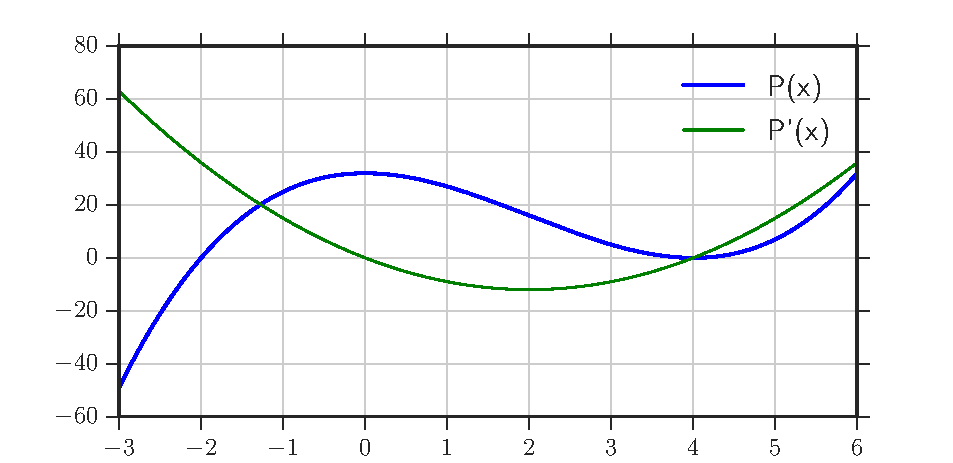
\includegraphics[width=\figwidth\linewidth]{figs/plot_1_d}
	\caption{Polynomet $P(x) = x^3 - 6x^2 + 32$ og den deriverte $P'(x) = 3x^2- 12x$.}
	\label{fig:plot1d}
\end{figure}
\end{easylist}

\subsection*{Oppgave 3}
Hver kvittering gir oss én likning. La oss bruke variabelnavn som gir mening i forhold til oppgaveteksten: en skolebolle er $s$, en bolle er $b$ og en muffin er $m$. Likningene våre blir seende slik ut:
\begin{align*}
	\text{Likning 1:   }\qquad& 4s + 4b +2m = 176 \\
	\text{Likning 2:   }\qquad& 2s + 4b +2m = 142 \\
	\text{Likning 3:   }\qquad& 3s + 5b +4m = 222 
\end{align*}
Det er alltid lurt å kikke litt på likningene før man løser, da har man større sjanse for å velge en grei fremgangsmåte.
Vi tar likning 1 minus liking 2. Da får vi \answer{$s = 17$}. Vi setter så dette inn i likning 2 og 3 slik at vi får følgende system:
\begin{align*}
\text{Likning A:   }\qquad& 4b +2m = 108 \\
\text{Likning B:   }\qquad& 5b + 4m = 171 
\end{align*}
Vi ganger så likning A med 2, deretter tar vi likning A minus likning B. Vi får da \answer{$b = 15$}. Sett inn $s$ og $b$ i hvilken som helst likning for å finne \answer{$m = 24$}. På eksamen er det stort sett alltid verdt tiden det tar å sette prøve på svaret.

\subsection*{Oppgave 4}
\begin{easylist}[enumerate]
	\ListProperties(Style2*=,Numbers=a,Numbers1=l,FinalMark={)})
	# Vi må regne ut følgende sum:
	\begin{equation*}
		16 + 17 + \dots + 19 + 30
	\end{equation*}
	Det er 15 ledd i denne summen. Vi bruker formelen for sum av en aritmetisk rekke, som er gitt av følgende formel:
	\begin{equation}
	\label{eqn:arit}
		S_n = \frac{a_1 + a_n}{2} \cdot n
	\end{equation}
	I formelen ovenfor er $a_1$ den første verdien, $a_n$ er den siste verdien og $n$ er antall ledd. Vi fyller inn det som gjelder for vår oppgave og får:
	\begin{equation*}
	S = \frac{a_1 + a_n}{2} \cdot n = \frac{16 + 30}{2} \cdot 15 = \answer{345}
	\end{equation*}
	
	# Det er $7-4 = 3$ differanser mellom $a_4$ og $a_7$, slik at $3d = 20-11 = 9$.
	Med andre ord må differansen $d$ være $3$. Vi vet at $a_n = a_0 + dn$, så vi kan finne $a_0$ ved å fylle inn det vi vet for $a_4$, nemlig at $a_4 = 11 = a_0 + 3(4)$, da er $a_0 = -1$ og vi får:
	\begin{equation*}
		a_n = a_0 + dn = -1 + 3n
	\end{equation*}
	Da er det bare å fylle inn for $n = 40$. Vi får $a_{40} = -1 + 3(40) = \answer{119}$.
\end{easylist}

\subsection*{Oppgave 5}
\begin{easylist}[enumerate]
	\ListProperties(Style2*=,Numbers=a,Numbers1=l,FinalMark={)})
	# Definisjonen av geometrisk rekke og aritmetisk rekke er:
	## En rekke $a_1 + a_2 + \dots + a_k + a_{k+1} + \dots$ er \emph{geometrisk} dersom forholdet $f = \frac{a_{k+1}}{a_k}$ er konstant for alle verdier av $k$. Kommentar: Geometriske rekker er en diskret variant av eksponentialfunksjoner $f(x) = Ce^{kx}$.
	## En rekke $a_1 + a_2 + \dots + a_k + a_{k+1} + \dots$ er \emph{aritmetisk} dersom differansen $d = a_{k+1} - a_k$ er konstant for alle verdier av $k$. Kommentar: aritmetiske rekker er en diskret variant av lineære funksjoner $f(x) = ax + b$.
	
	# Vi ser at det foregår en halvering for i hvert ledd, så vi ``gjetter'' at $a_k$ må være på formen $a_k = C \left(\frac{1}{2}\right)^k$, der $C$ er en ubestemt konstant. For å bestemme $C$ løser vi denne likningen:\footnote{Vi kunne brukt hvilket som helst ledd til å finne $C$, grunnen til at vi velger $a_2$ er helt tilfeldig.}
	\begin{equation*}
		a_2 = 5 = C \left(\frac{1}{2}\right)^2
	\end{equation*}
	Løsningen er at $C = 20$ slik at $a_k = 20 \left(\frac{1}{2}\right)^k = \answer{20/2^k}$. 
	
	# Vi regner ut $b_k$ fra definisjonen gitt i oppgaven:
	\begin{equation*}
		b_k = \ln \left(a_k\right) = \ln \left(\frac{20}{2^k}\right) = \ln(20) - k \ln(2)
	\end{equation*}
	Rekken er aritmetisk dersom differansen $d = b_{k+1} - b_k$ er konstant(uavhengig av indeksen $k$), så vi regner ut $d$ på følgende måte:
	\begin{align*}
	d = b_{k+1} - b_k &= \left[\ln(20) - (k+1) \ln(2)\right] - \left[\ln(20) - k \ln(2)\right] \\
					&=  - (k+1) \ln(2)  + k \ln(2) \\
					&=  - k \ln(2) - \ln(2)  + k \ln(2) \\
					&=\answer{- \ln(2)}
	\end{align*}
	\answer{Differansen $d$ er ikke avhengig av $k$, og da er rekken aritmetisk}.
	
\end{easylist}

\subsection*{Oppgave 6}
I denne oppgaven ser vi på funksjonen
\begin{equation*}
	f(x) = \ln \left(x^2 + 4\right)
\end{equation*}
\begin{easylist}[enumerate]
	\ListProperties(Style2*=,Numbers=a,Numbers1=l,FinalMark={)})
	# En funksjon $f(x)$ stiger når $f'(x)>0$ og synker når $f'(x)<0$. Vi bruker kjernereglen med $u = x^2 + 4$ og regelen $\ln(u)' = u' / u$ for å regne ut den deriverte av $f(x)$:
	\begin{equation*}
		f'(x) = \left( \ln \left(x^2 + 4\right) \right)' = \frac{\left(x^2 + 4\right)'}{x^2 + 4} =  \frac{2x}{x^2 + 4}
	\end{equation*}
	Nevneren $x^2 + 4$ er positiv for alle verdier av $x$, så vi trenger bare å se på telleren. Telleren er positiv når $x > 0$ og negativ når $x < 0$, så vi ser at funksjonen  \answer{stiger når $x > 0$ og synker når $x < 0$}.
	
	# Monotoniegenskapene (stigning og synking) passer ikke med figur A, så det må være B, C eller D.
	Vi ser på vendepunktene, altså når $f''(x)$ bytter fortegn, vi regner ut:
	\begin{equation*}
	f''(x) = \left(  2x  \left( x^2 + 4 \right)^{-1}  \right)' = ... = \frac{2}{x^2 + 4} - \frac{4x^2}{\left(x^2 + 4\right)^2} = \frac{ 8 -2x^2}{\left(x^2 + 4\right)^2}
	\end{equation*}
	Nevneren $\left(x^2 + 4\right)^2$ er alltid positiv, så vi ser på telleren. Den dobbelderiverte $f''(x)$ endrer fortegn når $x = \pm 2$. Dette stemmer best med \answer{figur C}, ettersom vi ser vendepunkter i nærheten av $\pm 2$.
\end{easylist}

\subsection*{Oppgave 7}
\begin{easylist}[enumerate]
	\ListProperties(Style2*=,Numbers=a,Numbers1=l,FinalMark={)})
	# Vi vet at summen av sannsynlighetene må være lik 1:
	\begin{equation*}
		\sum_{x \in X} P(X= x) = 1
	\end{equation*}
	I vårt tilfelle må $0,2 + 0,5 + a = 1$, og da må vi ha \answer{$a = 0,3$}.
	
	# Forventningsverdien $\mu = \operatorname{E}(X) = \sum_{x \in X} P(X =x)x$ blir her:
	\begin{equation*}
	\sum_{x \in X} P(X =x)x = 0 (0,2) + 10 (0,5) + 20 (0,3) = 5 + 6 = \answer{11}
	\end{equation*}
	Standardavviket $\sigma = \sqrt{\operatorname{Var}(X)}$ er litt mer vrient å regne ut uten kalkulator, men utregningen av variansen kan se omtrent slik ut:
	\begin{align*}
	\operatorname{Var}(X) &= \sum_{x \in X} P(X =x)(x - \mu)^2 \\
	&= 0,2(0-11)^2 + 0,5(10-11)^2 +  0,3(20-11)^2 \\
	&= 0,2(11)^2 + 0,5(-1)^2 +  0,3(9)^2 \\
	&= \frac{242}{10} + \frac{5}{10} +  \frac{3(81)}{10} \\
	&= \frac{242+5+243}{10} = \frac{490}{10} = 49 \\
	\end{align*}
	Da blir $\sigma = \sqrt{\operatorname{Var}(X)} = \sqrt{49} = \answer{7}$.
\end{easylist}

\subsection*{Oppgave 8}
\begin{easylist}[enumerate]
	\ListProperties(Style2*=,Numbers=a,Numbers1=l,FinalMark={)})
	# $P(22 < X < 42)$ er området mellom $22$ og $42$. I en sannsynlighetsfordeling er summen av arealet alltid lik 1, så det hvite området pluss de to blå områdene må være lik 1. Vi løser for det hvite området i likningen nedenfor:
	\begin{align*}
		\text{hvitt område} &+ 2 \times \text{blått område} = 1 \\
		\text{hvitt område} &+ 2 \times 0,106 = 1 \\
		\text{hvitt område} &= 1 - 2 \times 0,106 = 1-0,212 = \answer{0,788 }
	\end{align*}
	
	# En normalfordeling er symmetrisk rundt forventningsverdien $\mu$, som er $x$ verdien som samsvarer med ``toppen av fjellet.'' Ettersom de blå områdene er like store må $\mu$ ligge midt mellom 22 og 42:
	\begin{equation*}
		\mu = \frac{22 + 42}{2} = \answer{32}
	\end{equation*}
	
	# Fra tabellen ``Standard normalfordeling'' i vedlegg 1 kan vi lese at:
	\begin{equation*}
		P(Z < -1,25) = 0,1056 \approx 0,106
	\end{equation*}
	Området mellom $22$ og $\mu = 32$ inneholder altså omtrent $1,25$ standardavvik. Vi får likningen
	\begin{equation*}
		(32-22) = 1,25 \sigma 
	\end{equation*}
	som har løsning $\answer{\sigma = 8}$.\footnote{Et litt mer nøyaktig svar er $P(Z < -1,2481) = 0,106$, som gir $\sigma \approx 8,0123$.}
\end{easylist}




\section*{Del 2 - med hjelpemidler}
\subsection*{Oppgave 1}
\begin{easylist}[enumerate]
	\ListProperties(Style2*=,Numbers=a,Numbers1=l,FinalMark={)})
	# Det er lurt å lage et plot av datasettet i Geogebra for å se hvordan det ser ut. Skriv inn datasettet i regnearket, marker de to kolonnene,  høyreklikk og trykk ``Lag'' $\rightarrow$ ``Liste med punkt.'' Datasettet er plottet i figur \eqref{fig:oppgave1adel2}.
	\begin{figure}[th!]
		\centering
		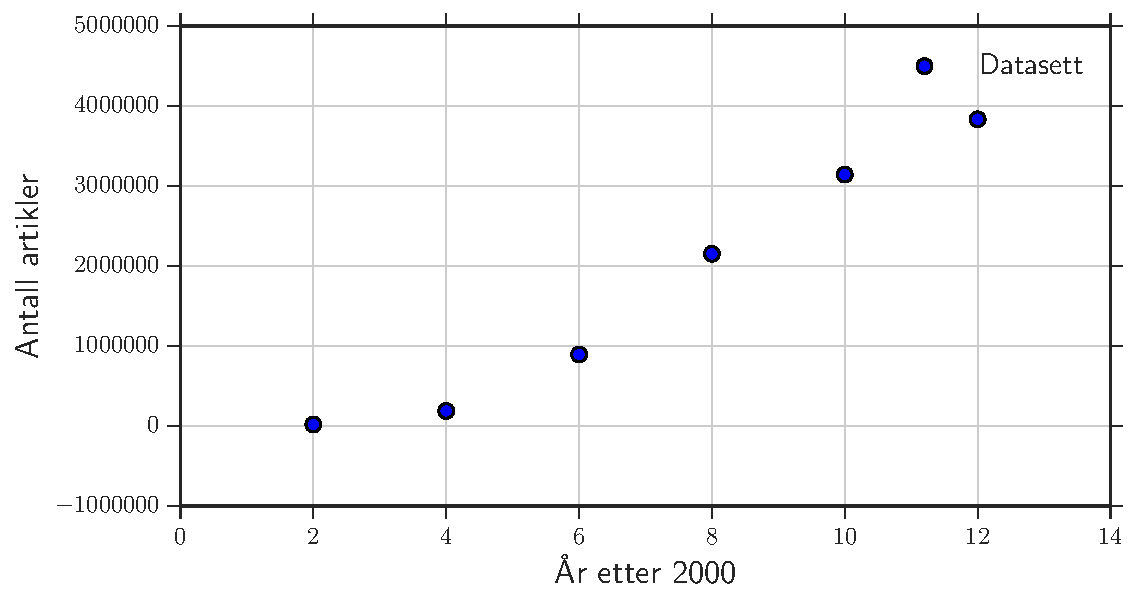
\includegraphics[width=\figwidth\linewidth]{figs/oppgave1_a_del2}
		\caption{Datasettet i oppgave 1a, del 2.}
		\label{fig:oppgave1adel2}
	\end{figure}
	## Vi kan forsøke med lineær regresjon først. 
	Vi bruker\footnote{Det er også mulig å markere data i regnearket og velge ``Regresjonsanalyse'', som er en knapp oppe til venstre på skjermen.} \\
	\texttt{RegLin[ <Liste med punkt> ]} \\
	kommandoen i Geogebra til å lage en lineær modell for datasettet:
	\begin{equation}
	\label{eqn:lin_model}
		f(x) = 417144x - 1214093
	\end{equation}
	I figur \eqref{fig:oppgave1_a_del2_lin} ser vi datasettet, samt den lineære modellen gitt av likning \eqref{eqn:lin_model}.
	\begin{figure}[th!]
		\centering
		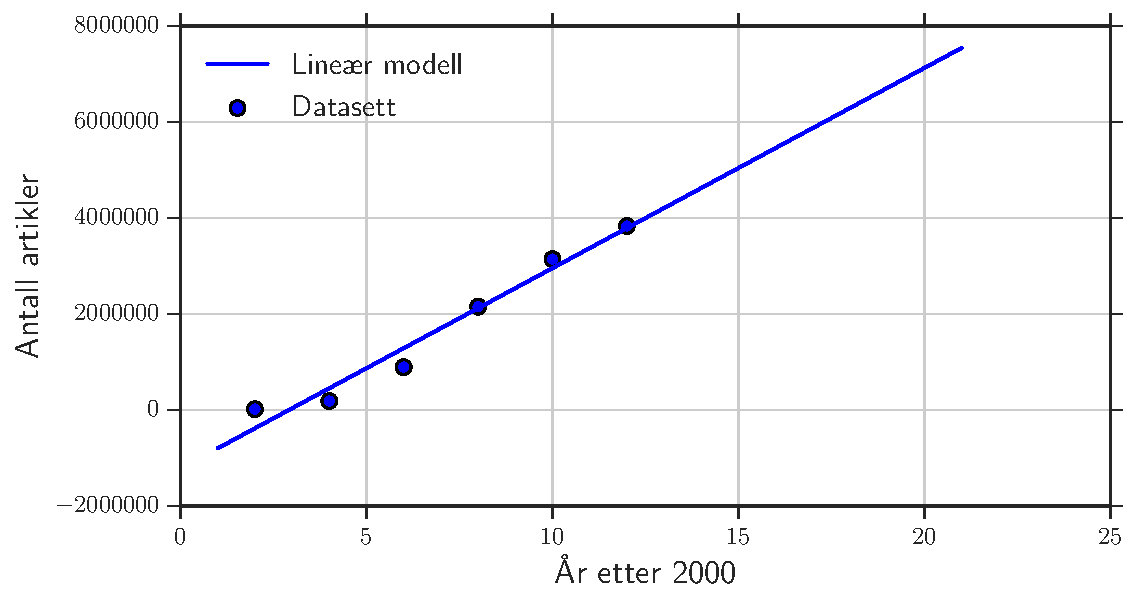
\includegraphics[width=\figwidth\linewidth]{figs/oppgave1_a_del2_lin}
		\caption{Datasettet i oppgave 1a, del 2 og den lineære modellen.}
		\label{fig:oppgave1_a_del2_lin}
	\end{figure}
	Vi har at $f(20) = 7,13$ millioner, noe som samsvarer godt med journalistens påstand om at det vil være rundt 7 millioner artikler på Wikipedia i år 2020. En av modellene er altså en \answer{lineær modell}.

	## La oss undersøke en logistisk modell. 
	Vi bruker \\
	\texttt{RegLogist[ <Liste med punkt> ]} \\
	kommandoen i Geogebra til å lage en logistisk modell for datasettet, og får dette som svar:
	\begin{equation}
	\label{eqn:log_model}
	g(x) = \frac{4008254}{1 + 211,4052e^{-0,6801x}}
	\end{equation}
	I figur \eqref{fig:oppgave1_a_del2_log} ser vi datasettet samt en logistisk modell gitt av likning \eqref{eqn:log_model}.
	Legg merke til at når $x \to \infty$ så vil $g(x) \to 4008254 \approx 4000000$. 
	Den andre journalisten har brukt en \answer{logistisk modell} når han/hun har kommet frem til at antall artikler vil stabilisere seg på rundt 4 millioner.
	\begin{figure}[th!]
		\centering
		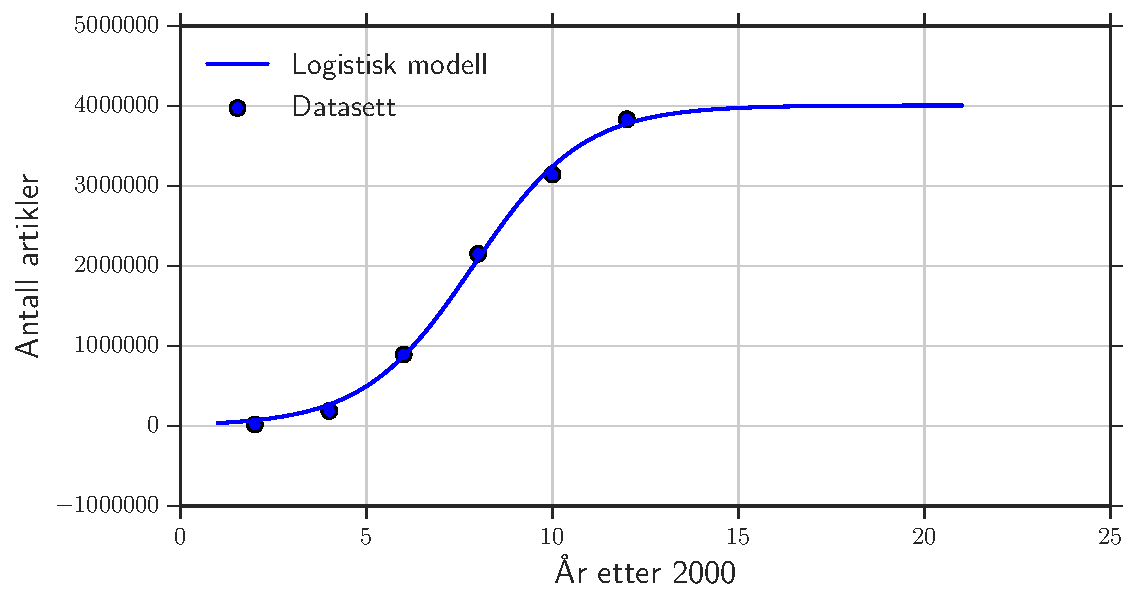
\includegraphics[width=\figwidth\linewidth]{figs/oppgave1_a_del2_log}
		\caption{Datasettet i oppgave 1a, del 2 og den logistiske modellen.}
		\label{fig:oppgave1_a_del2_log}
	\end{figure}
	
	# Stor vekst skjer når den deriverte, $g'(x)$, er høy.
	Den største veksten skjer når $g'(x)$ er høyest. 
	Vi må altså finne toppunktet til $g'(x)$.
	Dette gjør vi ved å tegne funksjonen i Geogebra og bruke \\
	\texttt{Maks[ <Funksjon>, <Start x-verdi>, <Slutt x-verdi> ]}\\ 
	Da får vi punktet $(7.87, 0.68)$, det vil si at året der antall artikler vokste raskest er $2007.87 \approx \answer{2007}$. Funksjonen $g'(x)$ er plottet i figur \eqref{fig:oppgave1_b_del2}.
	\begin{figure}[th!]
		\centering
		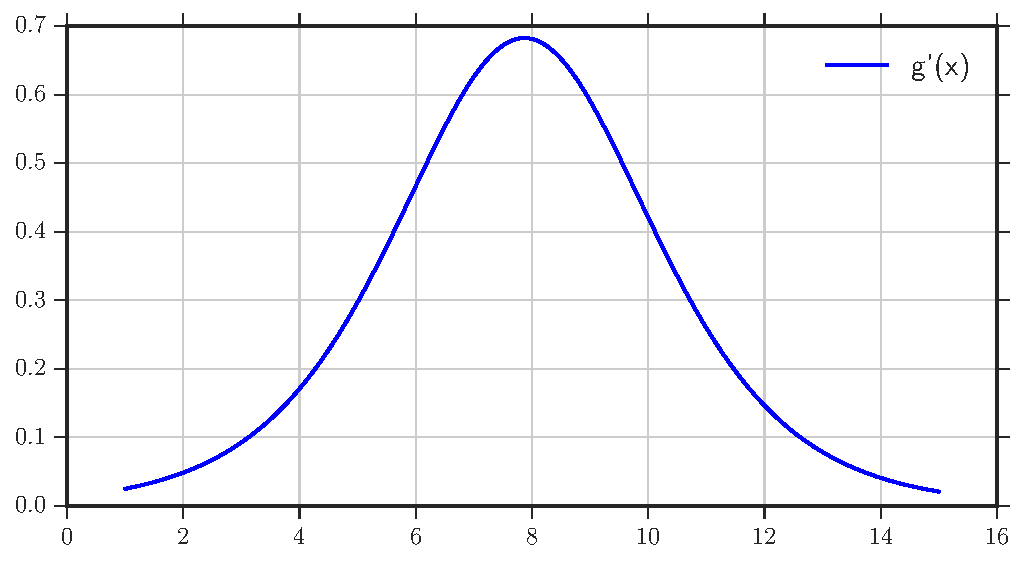
\includegraphics[width=\figwidth\linewidth]{figs/oppgave1_b_del2}
		\caption{Grafen til $g'(x)$ i oppgave 1b, del 2.}
		\label{fig:oppgave1_b_del2}
	\end{figure}

	# Vi bruker \\
	\texttt{Integral[ <Funksjon>, <Start>, <Slutt> ]}\\
	kommandoen til å regne ut integralet. Dersom funksjonen er definert som \texttt{g(x)} kan vi skrive: \\
	\texttt{a = Integral[g, 0, 15]} \\
	Da får vi vite at arealet $a \approx \answer{3,96}$. Forholdet mellom den deriverte $g'(x)$ og et integral er gitt ved:\footnote{Dette er \emph{fundamentalteoremet i kalkulus}.}
	\begin{equation*}
		\int_{a}^{b} g'(x) \ dx = g(b) - g(a)
	\end{equation*}
	I vårt tilfelle er tolkningen av $\int_{0}^{15} g'(x) \ dx = g(15) - g(0)$ den totale endringen i artikler fra 2000 til 2015.
	


\end{easylist}

\subsection*{Oppgave 2}
\begin{easylist}[enumerate]
	\ListProperties(Style2*=,Numbers=a,Numbers1=l,FinalMark={)})
	# Likningssettet er:
	\begin{align*}
		K(50) &= 3225 \\
		K(100) &= 4900 \\
		K'(100) &= 41 
	\end{align*}
	Følgende kommando i CAS i Geogebra løser likningssettet, her skrevet over flere linjer for å være lettere å lese:\footnote{Det er kanskje lettest å skrive lange kommandoer i notepad og lime inn i CAS etterpå, i tilfelle du skriver feil eller trykker på noe i Geogebra slik at alt forsvinner.} \\
	\texttt{Løs[\\
		\{a(50)\textasciicircum2 + b(50) + c = 3225, \\ 
		a(100)\textasciicircum2 + b(100) + c = 4900, \\ 
		2a(100) + b = 41\}, \\
		\{a, b, c\}\\
		]} \\
	Løsningen er $\answer{a = 3/20}$, $\answer{b = 11}$ og $\answer{c = 2300}$. Funksjonen $K(x)$ blir da:
	\begin{equation*}
	K(x) = ax^2 + bx + c = \frac{3}{20}x^2 + 11x + 2300
	\end{equation*}
	Vi kan derivere $K(x)$ ovenfor for å bekrefte at $\answer{K'(x) = (3/10)x + 11}$.
	
	# Vi kan derivere $I(x)$ og $K(x)$ for hånd eller med CAS, da får vi:
	\begin{align*}
		I'(x) & = 31,87 \\
		K'(x) & = 41
	\end{align*}
	$I'(x)$ forteller oss hvor mye mer vi får i inntekt (per enhet $x$) dersom vi produserer én enhet mer. På samme måte forteller $K'(x)$ oss hvor mye mer kostnadene blir (per enhet $x$) dersom vi produserer én enhet mer.
	Bedriften bør produsere \answer{færre enn 100 enheter}, ettersom grensekostnadene overstiger grenseinntektene når $x = 100$.
	Legg merke til at overskuddet er $O(x) = I(x) - K(x)$, slik at $O'(x) = I'(x) - K'(x)$.
	Dersom $K'(x) > I'(x)$ er $O'(x) < 0$, og overskuddet synker når vi øker $x$. Vi vil selvsagt ikke produsere mer i en slik situasjon.
	
	# Vi definerer overskuddet som inntekt minus kostnad $O(x) = I(x) - K(x)$. Overskuddet blir
	\begin{equation*}
		O(x) = 3200 \ln \left(2,5x + 1\right) - \left( \frac{3}{20}x^2 + 11x + 2300 \right)
	\end{equation*}
	For å løse oppgaven plotter vi $O(x)$ i Geogebra og kjører følgende kommando: \\
	\texttt{Maks[ <Funksjon>, <Start x-verdi>, <Slutt x-verdi> ]}\\
	Svaret er at bedriften må produsere og selge $86,33 \approx$ \answer{86 enheter per dag} for å oppnå et maksimalt overskudd.
	Funksjonen $O(x)$ er plottet i figur \eqref{fig:oppgave2c}.
\begin{figure}[th!]
	\centering
	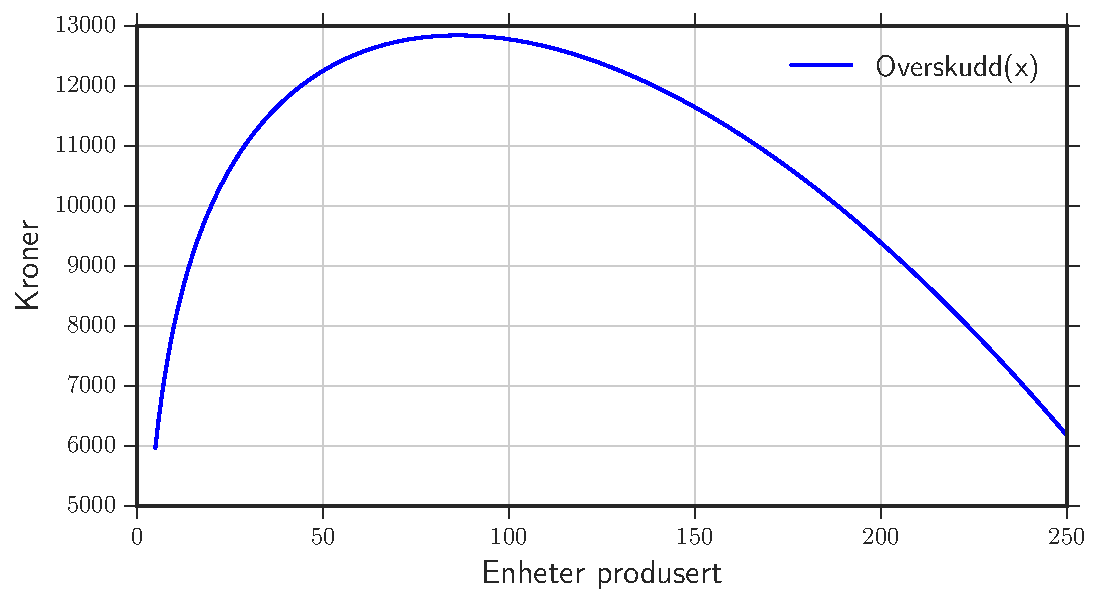
\includegraphics[width=\figwidth\linewidth]{figs/oppgave2_c}
	\caption{Et plot av $O(x)$ fra oppgave 2c, del 2.}
	\label{fig:oppgave2c}
\end{figure}
\end{easylist}

\subsection*{Oppgave 3}
\begin{easylist}[enumerate]
	\ListProperties(Style2*=,Numbers=a,Numbers1=l,FinalMark={)})
	# I utgangspunktet er den stokastiske variabelen $x$ binomisk fordelt med $n = 1000$ og $p = 0,308$, men dersom $np > 5$ og $n(1-p) >5$ kan vi approksimere den binomiske fordelingen med en normalfordeling. Ettersom $np = 308 > 5 $ og $n(1-p) = 692 >5$ vil normalfordelingen her være en god approksimasjon. Se figur \eqref{fig:oppgave3plot} for et plot som viser hvor god denne approksimasjonen er (veldig god her, siden både $np$ og $n(1-p)$ er mye større enn 5).
	

	\begin{figure}[th!]
		\centering
		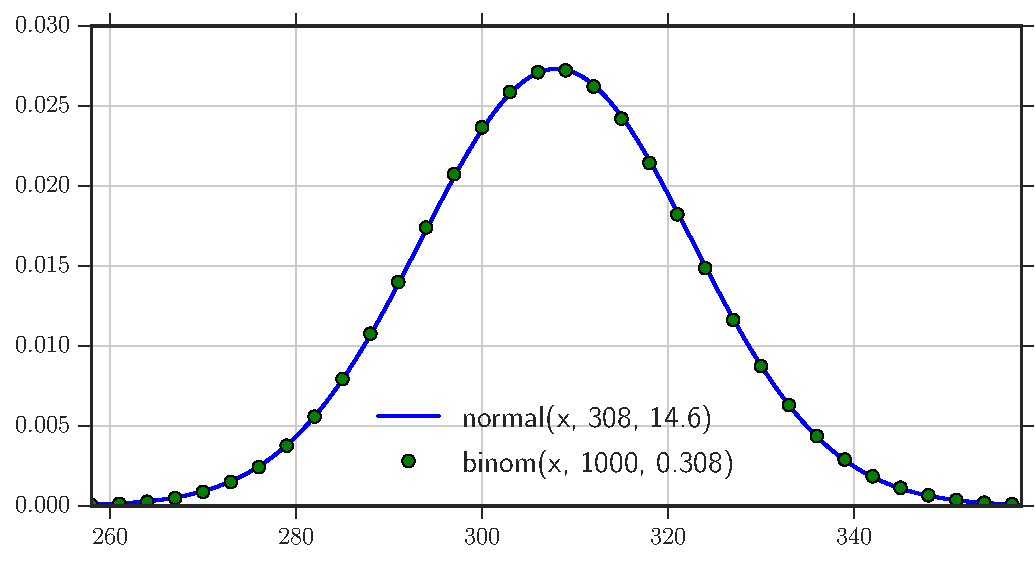
\includegraphics[width=\figwidth\linewidth]{figs/oppgave3_plot}
		\caption{Binomisk fordeling og normalfordeling i oppgave 3a, del 2.}
		\label{fig:oppgave3plot}
	\end{figure}
	# For en binomisk fordeling får vi følgende utregninger:
	\begin{align*}
		\mu &= \operatorname{E}(X) = np = 1000(0,308) = \answer{308} \\
		\sigma &= \sqrt{\operatorname{Var}(X)} = \sqrt{np(1-p)} \\
		&= \sqrt{1000(0,308)(1-0,308)} = \sqrt{213,136} \approx \answer{14,6}
	\end{align*}
	
	# La $X$ være antall personer i spørreundersøkelsen som ville ha stemt på partiet.
	Vi setter opp følgende hypoteser:
	\begin{align*}
		H_0 &: \quad p = 0,308  \\
		H_1 &: \quad p > 0,308
	\end{align*}
	Den observerte verdien er $x_{\text{obs}} = 334$. $P$-verdien er sannsynligheten for et så ekstremt resultat som den observerte verdien, eller endra mer ekstremt, gitt at $H_0$ er sann. Med andre ord er $P$-verdien sannsynligheten for å få $X \geq x_{\text{obs}}$ gitt at $H_0$ er sann. Vi kan regne ut $P$-verdien på 2 måter:
	\begin{easylist}[enumerate]
	## Vi kan bruke binomisk fordeling. Sannsynligheten for at $X \geq x_{\text{obs}} = 334$ gitt at $p = 0,308$ er $0,0411$. Utregningen gjør vi i sannsynlighetskalkulatoren til Geogebra.
	## Vi kan bruke normalfordelingen til å tilnærme den binomisk fordelingen. Når $p = 0,308$ og $n=1000$ har vi allerede regnet ut $\mu = 308$ og $\sigma = 14,6$. Vi får at $P$-verdien blir $P(333,5 \leq X) = 0,0404$. Dette tallet er også fra sannsynlighetskalkulatoren. Legg også merke til heltallskorreksjonen når vi går fra en diskret til en kontinuerlig sannsynlighetsfordeling.
\end{easylist}
	Uansett hvilken metode vi velger får vi at $P$-verdien er mindre enn 0,05, så \answer{vi forkaster $H_0$}, og vi har grunnlag for å si at oppslutningen til partiet har økt.
	
\end{easylist}

\subsection*{Oppgave 4}
\begin{easylist}[enumerate]
	\ListProperties(Style2*=,Numbers=a,Numbers1=l,FinalMark={)})
	# Vi løser likningen $b\times (1.025)^{18} = 100000$ for beløpet $b$, svaret blir:
	\begin{equation*}
		b = \frac{100000}{(1.025)^{18}} = 64116.591 \approx \answer{64117}
	\end{equation*}
	# Vi tolker oppgaven som følger:
	\begin{easylist}
		## Ole Magnus får første beløp på dagen han blir født. 
		## Han får 18 beløp til sammen. 
		Da får han siste beløp når han fyller 17. 
		Vi regner med at han får renter fra 17 årsdagen til 18 årsdagen,
		men har får ikke et beløp på 18 årsdagen---da ville han fått 19 beløp til sammen.
	\end{easylist} 
	La oss se på litt generell teori.
	Pengene $T$ etter $n$ år kan skrives slik, der $r$ er rente og $b$ er årlig beløp:
	\begin{align*}
		T_0 &= b \\
		T_1 &= br + b \\
		T_2 &= br^2 + br + b \\
		\ldots &= \ldots \\
		T_n &= b  \underbrace{ \left( r^n + r^{n-1} + \dots + 1 \right)}_{n+1\text{ ledd i summen}}   \\
		T_n &= b  \left( \frac{r^{n+1}-1}{r-1} \right)   
	\end{align*}
	Fra nest siste til siste linje bruker vi summeformelen for geometriske rekker.
	
	Etter 17 år har Ole Magnus $T_{17}$, deretter får han renter én gang, og etterpå skal han ha 100000 kroner. 
	Dette gir likningen $T_{17}r = 100000$. Vi kan skrive og løse den slik
	\begin{equation*}
		T_{17}r = 100000 
		\quad \Rightarrow \quad
		b  \left( \frac{r^{17+1}-1}{r-1} \right) r = 100000
		\quad \Rightarrow \quad
		b = \frac{100000(r-1)}{r(r^{17+1}-1)}
	\end{equation*}
	Setter vi inn tallene og løser får vi $\answer{b = 4358.06}$.
	
	Denne oppgaven kan løses uten PC, men oppgaven ber oss om å løse i CAS i Geogebra. For å løse i CAS skriver vi inn følgende: \\
	\texttt{NLøs[Sum[b * 1.025\textasciicircum x, x, 0, 17] * 1.025 = 100000]} \\
	Som løser følgende likning for oss:
	\begin{equation*}
		100000 = \underbrace{\left( b \sum_{x=0}^{18} (1,025)^x \right)}_{T_{17} = \text{penger etter 17 år}} \times r
	\end{equation*}
	Svaret blir det samme. På eksamen er det lurt å kladde litt på ark først, men det er raskere å løse i CAS enn å bruke summeformelen for en geometrisk rekke.
	
	# Igjen antar vi at første innbetaling $b$ blir gjort når Ole Magnus blir født, samt at siste innbetaling blir gjort på 17 årsdagen.
	Vi begynner med år 0 og lager en tabell, der vi setter økningen i beløpet til $o = 1.02$.
	Den rekursive formelen er $T_n = T_{n-1}r + bo^n$, altså ``forrige verdi ganget med rente, pluss et nytt beløp som øker hvert år.''
	Vi kan sette opp en tabell og undersøke situasjonen slik:
	\begin{center}
		\begin{tabular}{l|l|l}
			\textbf{År} & \textbf{Uttrykk} & \textbf{Pent uttrykk} \\ \hline
			0 & $b$ & $b$ \\
			1 & $br + bo$ & $b(r+o)$ \\
			2 & $\left(br + bo\right)r + bo^2$ & $b(r^2 + ro + o^2)$ \\
			3 & $\left( \left(br + bo\right)r + bo^2 \right)r + bo^3$ & $b(r^3 + r^2o + ro^2 + o^3)$ \\
			$\vdots$ & $\vdots$ & $\vdots$ \\
			$n$ & $\dots$ & $b \sum_{x = 0}^{n} o^x r^{n-x}$
		\end{tabular}
	\end{center}
	Vi ser mønsteret i høyre kolonne av tabellen.
	Igjen blir vi bedt om å løse problemet i CAS i Geogebra, så vi skriver inn: \\
	\texttt{o := 1.02} \\
	\texttt{r := 1.025} \\
	\texttt{Nløs[b * Sum[o\textasciicircum x * r\textasciicircum(17 - x), x, 0, 17] * r = 100000]} \\
	Løsningen blir $b = \answer{3712.01}$. I figur \eqref{fig:oppgave4plot2} ser vi grafer for hele oppgave 4, legg merke til at etter 18 år har Ole Magnus 100000 kroner i alle tilfellene. 
	\begin{figure}[th!]
		\centering
		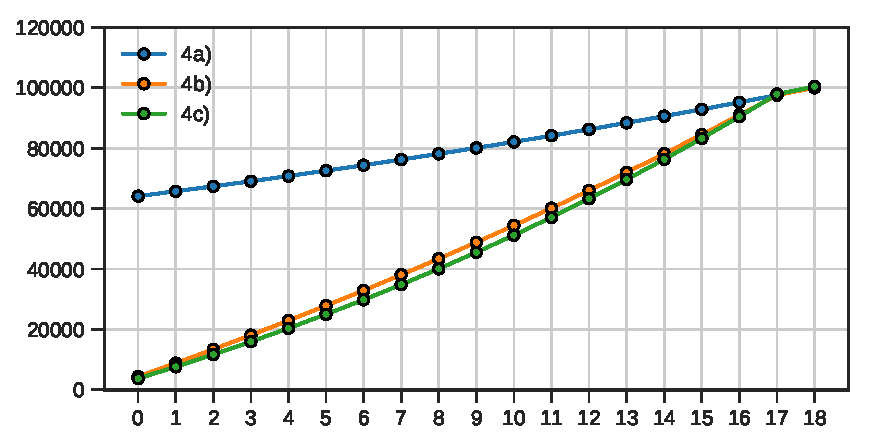
\includegraphics[width=\figwidth\linewidth]{figs/oppgave4_plot2}
		\caption{Scenarioer fra oppgave 4, del 2.}
		\label{fig:oppgave4plot2}
	\end{figure}
\end{easylist}




\end{document}


